
\section{Stromkreis}
\label{section:stromkreis}
\begin{frame}%STARTCONTENT

\begin{columns}
    \begin{column}{0.48\textwidth}
    \begin{itemize}
  \item Besteht aus einer Spannungsquelle und einem Verbraucher
  \item Die Spannung bringt den Strom zum Fließen
  \end{itemize}

    \end{column}
   \begin{column}{0.48\textwidth}
       
\begin{figure}
    \DARCimage{0.85\linewidth}{662include}
    \caption{\scriptsize Geschlossener Stromkreis}
    \label{n_stromkreis_geschlossen}
\end{figure}


   \end{column}
\end{columns}

\end{frame}

\begin{frame}
\frametitle{Schalter}
\begin{columns}
    \begin{column}{0.48\textwidth}
    \begin{itemize}
  \item Unterbricht oder schließt Stromkreis
  \item Bei offenem Schalter ist der Stromfluss unterbrochen
  \end{itemize}

\begin{figure}
    \DARCimage{0.85\linewidth}{663include}
    \caption{\scriptsize Offener Stromkreis}
    \label{n_stromkreis_offen}
\end{figure}


    \end{column}
   \begin{column}{0.48\textwidth}
       
\begin{figure}
    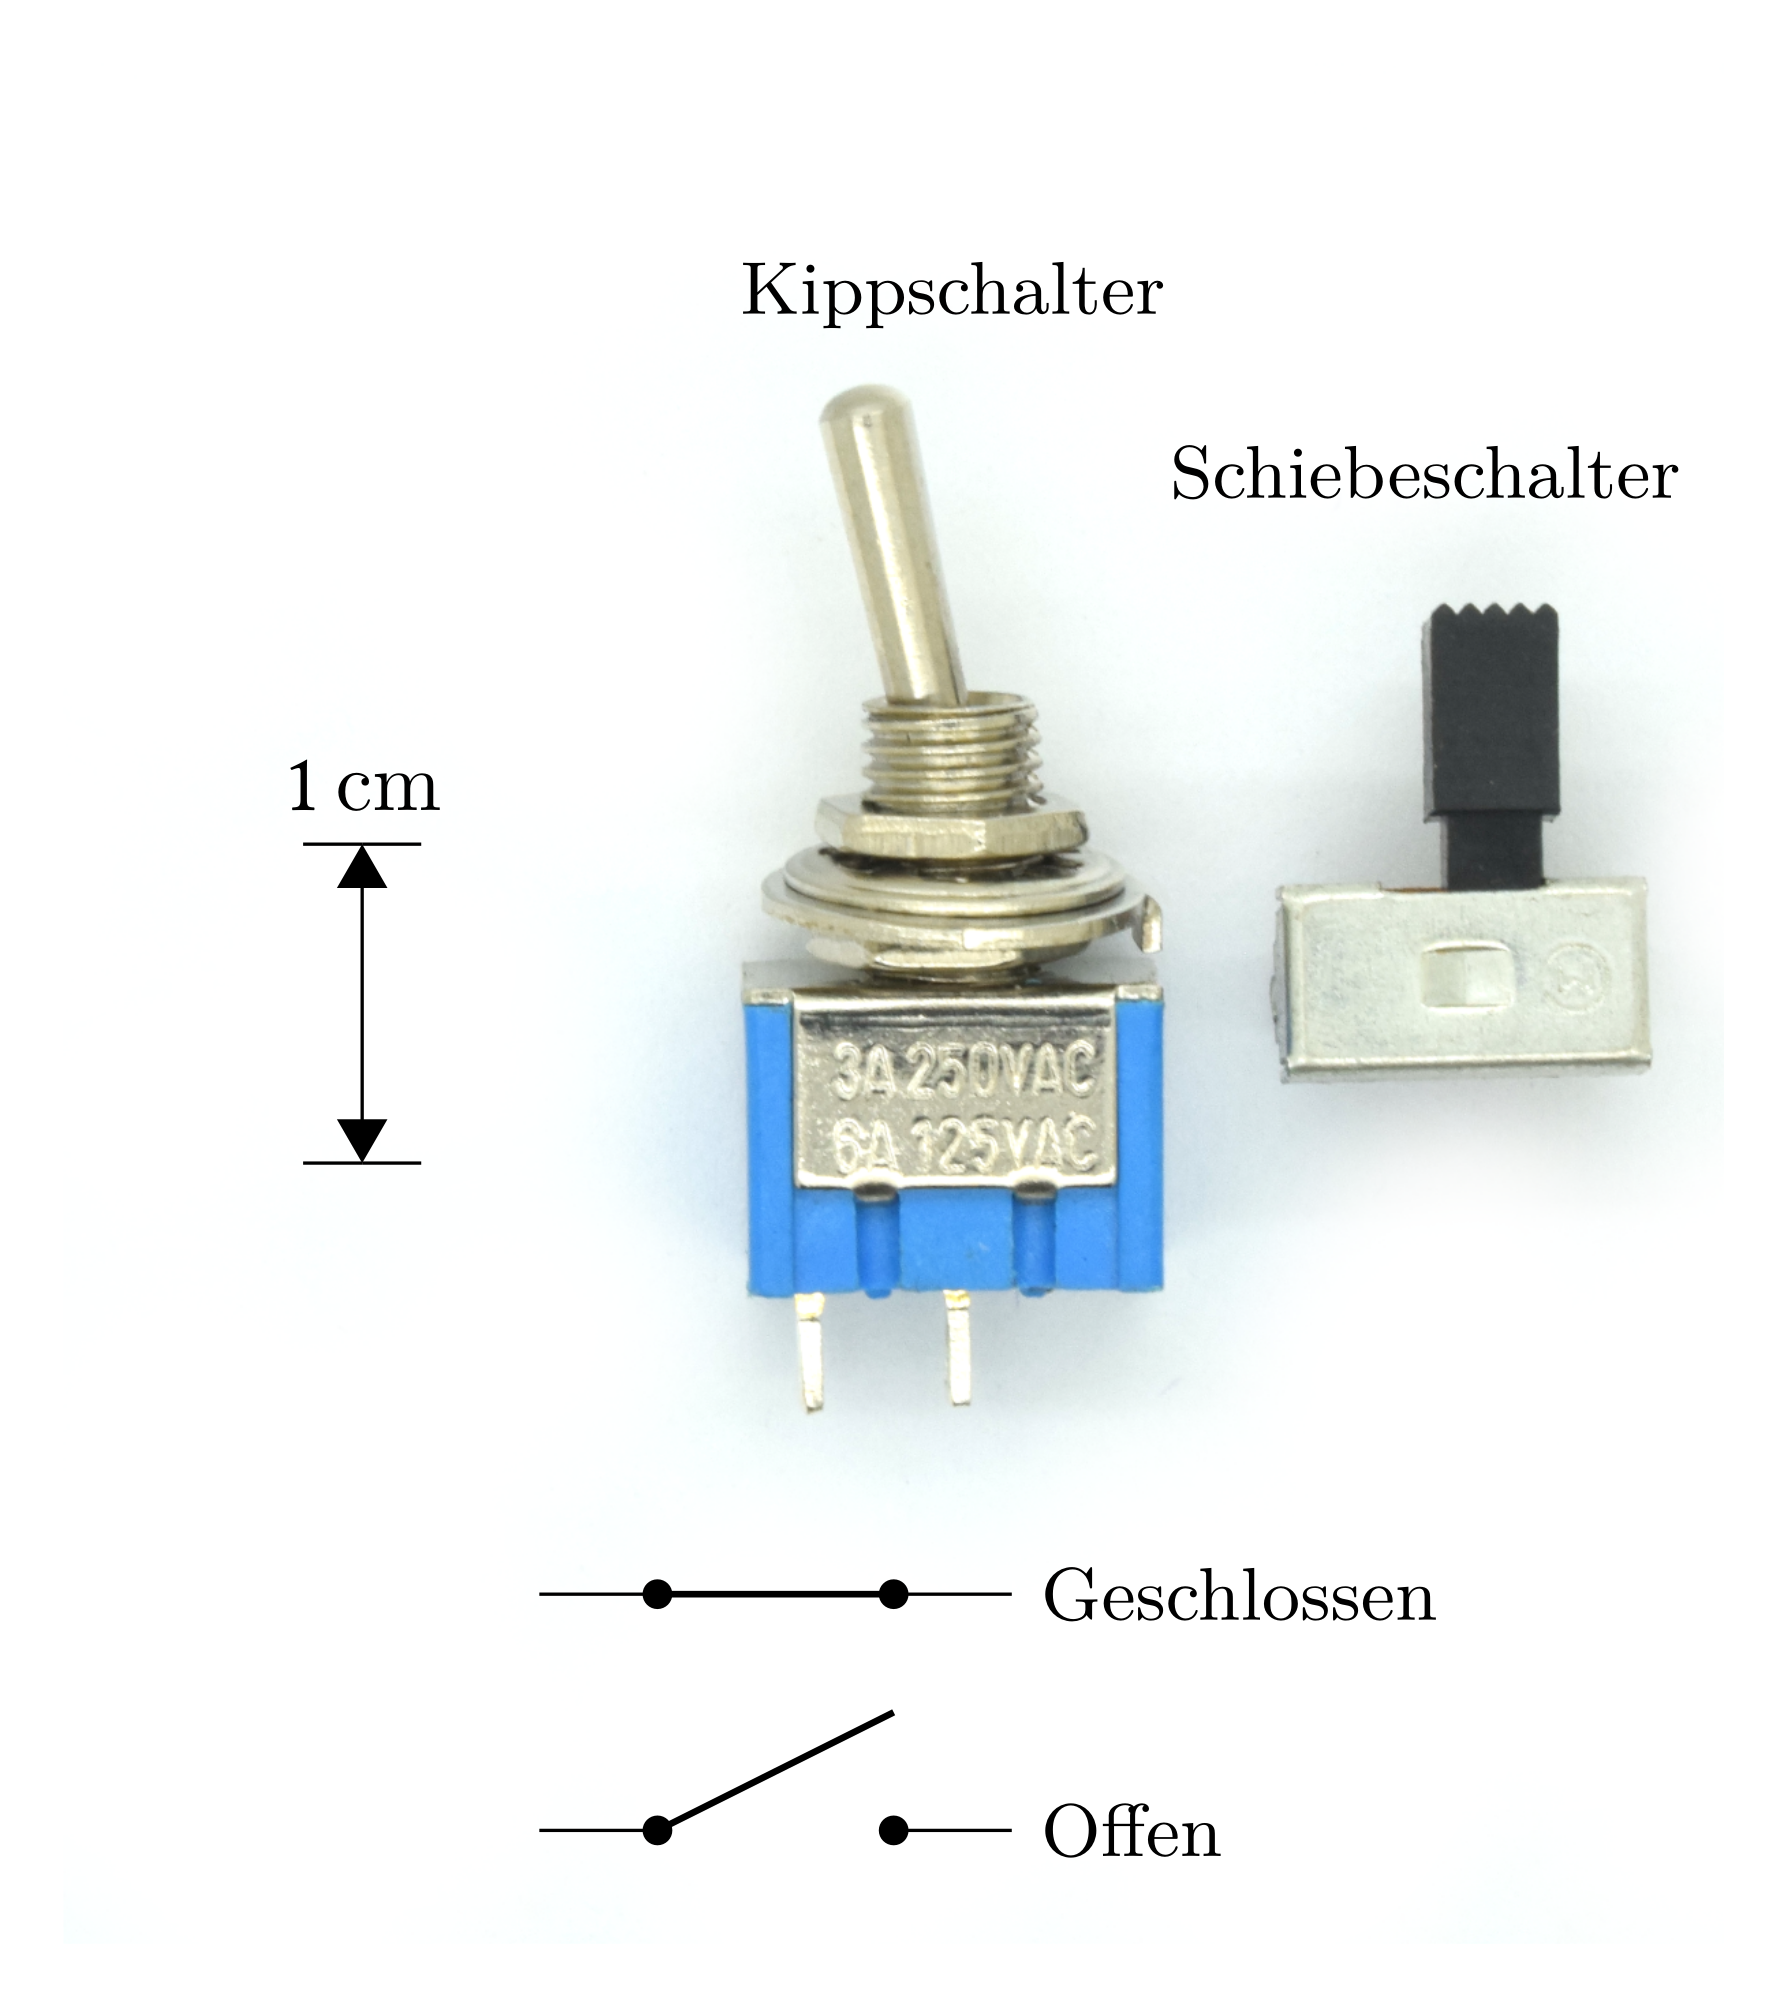
\includegraphics[width=0.85\textwidth]{foto/202}
    \caption{\scriptsize Schaltzeichen und Bauformen von Schaltern}
    \label{n_stromkreis_schalter}
\end{figure}

   \end{column}
\end{columns}

\end{frame}

\begin{frame}
\only<1>{
\begin{PQuestion}{NB701}{Welches Bauteil wird durch das Schaltzeichen symbolisiert?}{Masse}
{Schalter}
{Antenne}
{Erde}
{\DARCimage{0.5\linewidth}{546include}}\end{PQuestion}

}
\only<2>{
\begin{PQuestion}{NB701}{Welches Bauteil wird durch das Schaltzeichen symbolisiert?}{Masse}
{\textbf{\textcolor{DARCgreen}{Schalter}}}
{Antenne}
{Erde}
{\DARCimage{0.5\linewidth}{546include}}\end{PQuestion}

}
\end{frame}

\begin{frame}
\frametitle{Widerstand}
\begin{columns}
    \begin{column}{0.48\textwidth}
    \begin{itemize}
  \item Begrenzt den Stromfluss
  \item Wandelt Strom in Wärme um
  \end{itemize}

    \end{column}
   \begin{column}{0.48\textwidth}
       
\begin{figure}
    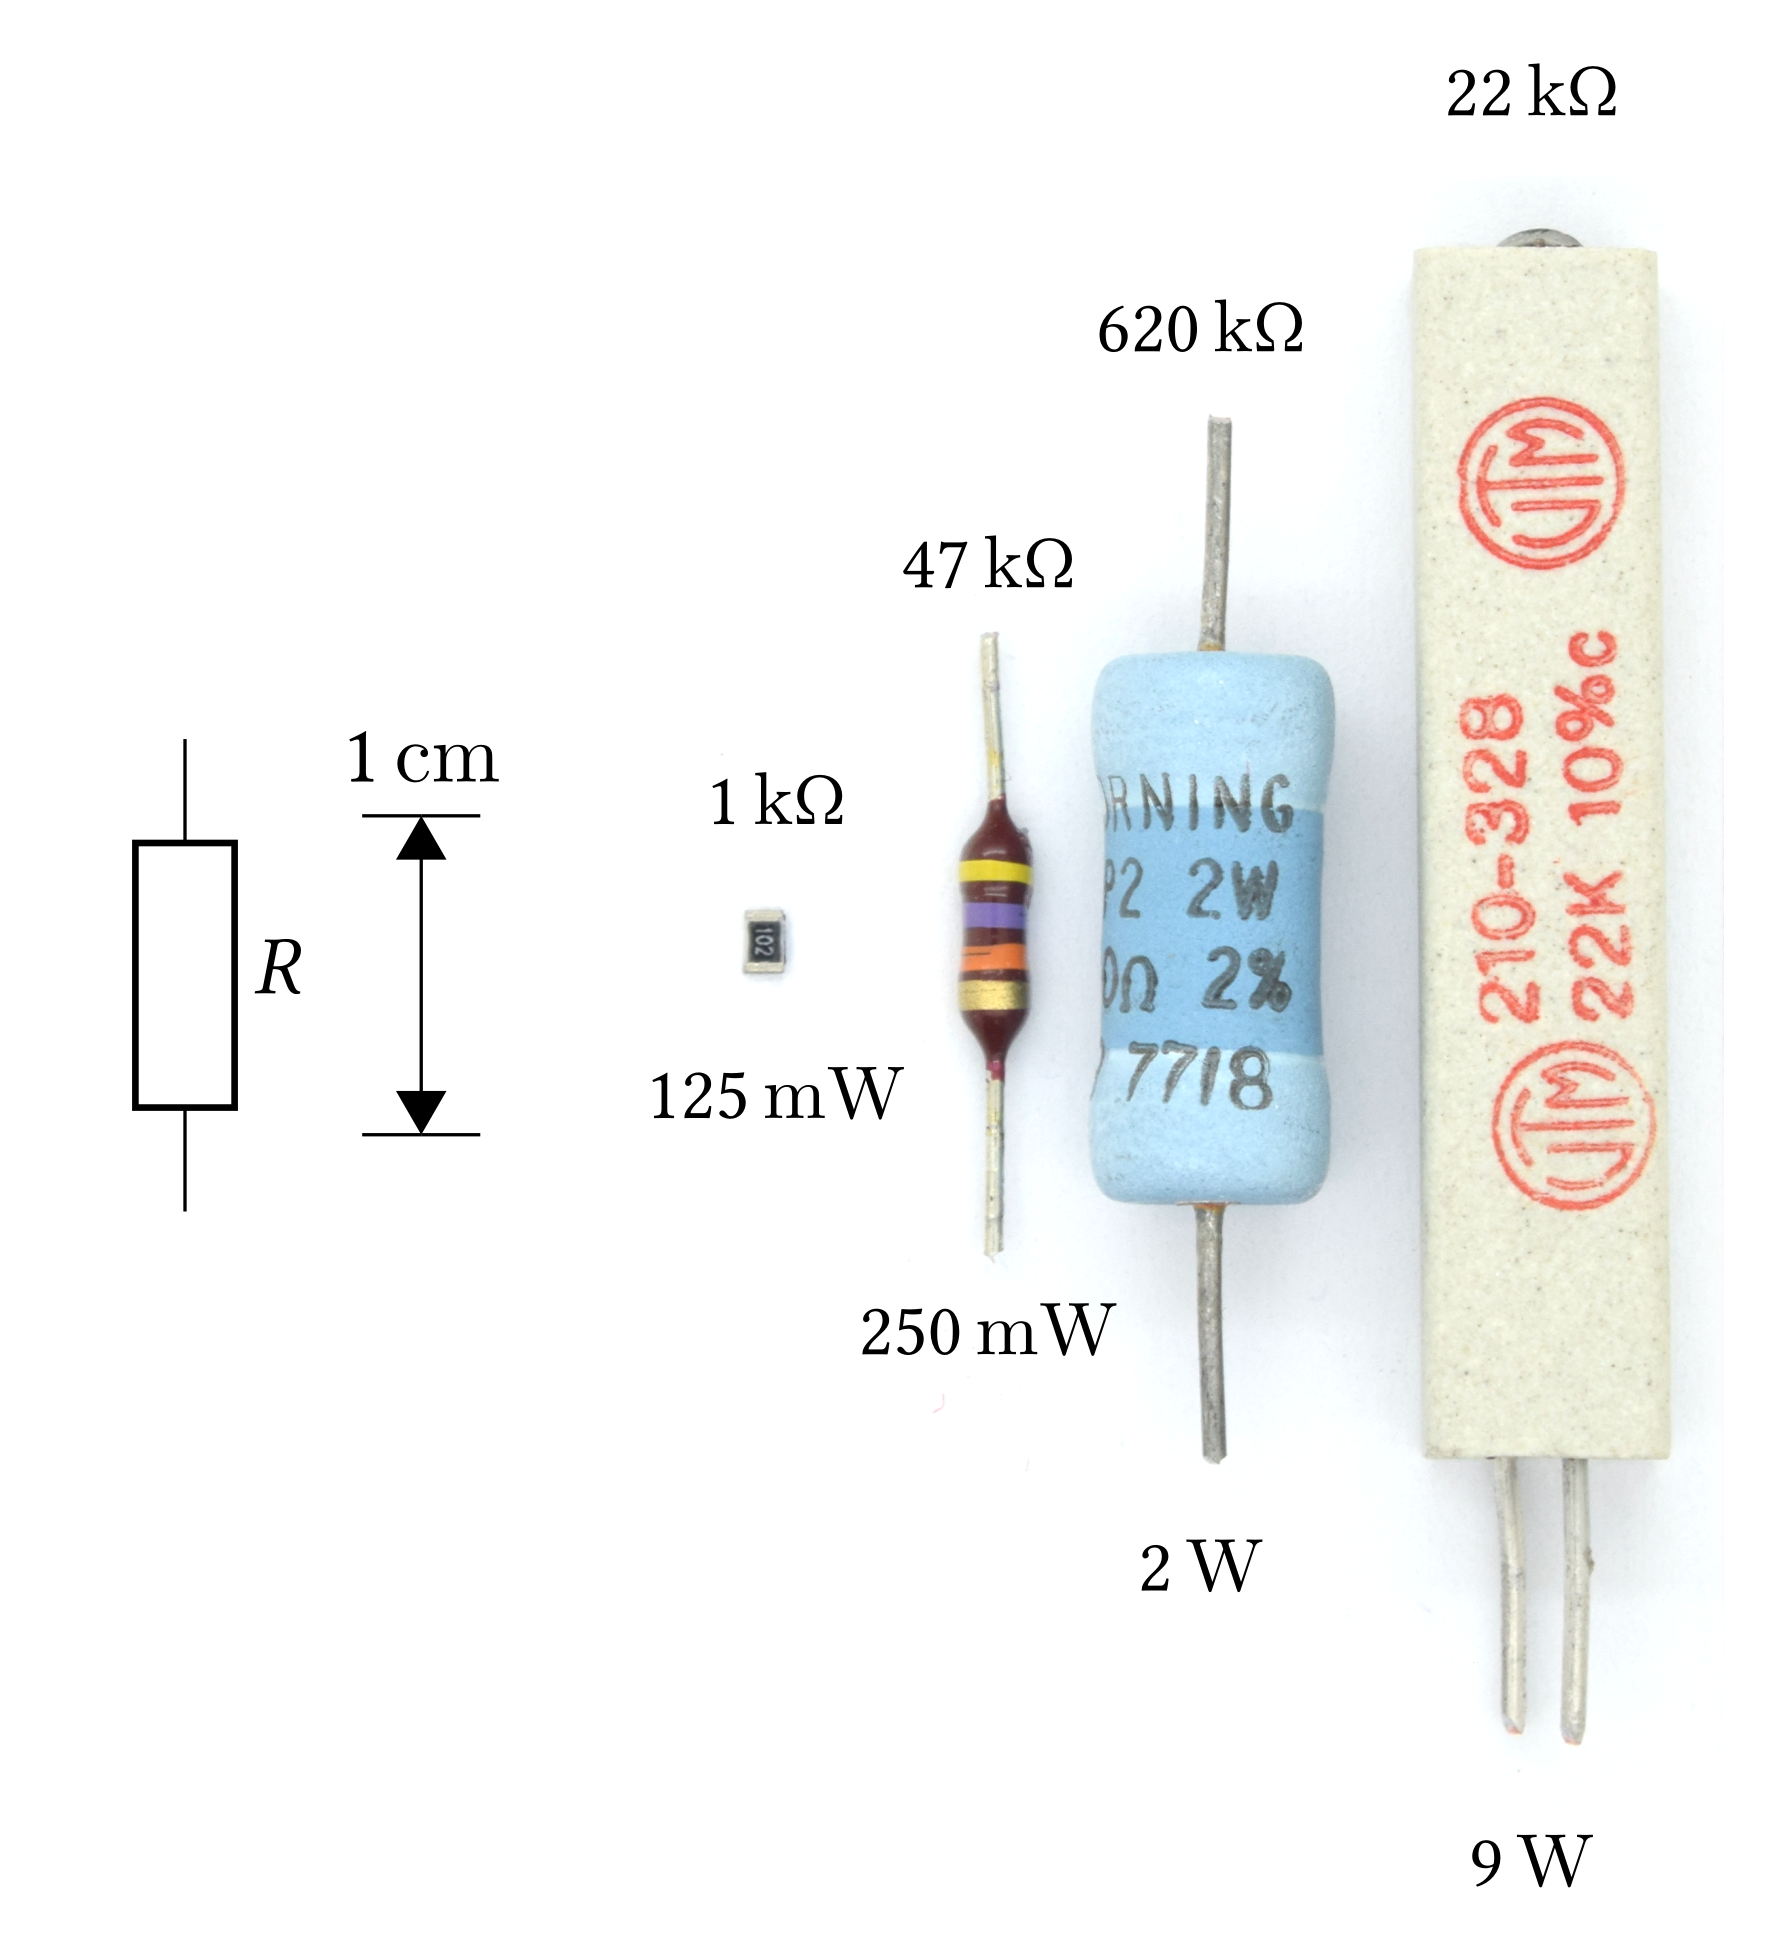
\includegraphics[width=0.85\textwidth]{foto/203}
    \caption{\scriptsize Schaltzeichen und Bauformen von Widerständen}
    \label{n_stromkreis_widerstand}
\end{figure}

   \end{column}
\end{columns}

\end{frame}

\begin{frame}
\only<1>{
\begin{PQuestion}{NC101}{Welches Bauteil wird durch das Schaltzeichen symbolisiert?}{Kondensator}
{Diode}
{Spule}
{Widerstand}
{\DARCimage{0.5\linewidth}{509include}}\end{PQuestion}

}
\only<2>{
\begin{PQuestion}{NC101}{Welches Bauteil wird durch das Schaltzeichen symbolisiert?}{Kondensator}
{Diode}
{Spule}
{\textbf{\textcolor{DARCgreen}{Widerstand}}}
{\DARCimage{0.5\linewidth}{509include}}\end{PQuestion}

}
\end{frame}

\begin{frame}
\frametitle{Stromrichtung}

\begin{figure}
    \DARCimage{0.85\linewidth}{662include}
    \caption{\scriptsize Geschlossener Stromkreis}
    \label{n_stromkreis_geschlossen}
\end{figure}

Vom Pluspol zum Minuspol: \emph{technische Stromrichtung}

\end{frame}

\begin{frame}
\only<1>{
\begin{question2x2}{NB702}{Welches Bild zeigt die technische Stromrichtung korrekt an?}{\DARCimage{1.0\linewidth}{536include}}
{\DARCimage{1.0\linewidth}{535include}}
{\DARCimage{1.0\linewidth}{537include}}
{\DARCimage{1.0\linewidth}{538include}}
\end{question2x2}

}
\only<2>{
\begin{question2x2}{NB702}{Welches Bild zeigt die technische Stromrichtung korrekt an?}{\DARCimage{1.0\linewidth}{536include}}
{\textbf{\textcolor{DARCgreen}{\DARCimage{1.0\linewidth}{535include}}}}
{\DARCimage{1.0\linewidth}{537include}}
{\DARCimage{1.0\linewidth}{538include}}
\end{question2x2}

}
\end{frame}

\begin{frame}
\only<1>{
\begin{PQuestion}{NB207}{Kann in folgender Schaltung von zwei gleichen Spannungsquellen Strom fließen? Welche Begründung ist richtig?}{Ja, weil der Pluspol mit dem Minuspol verbunden ist.}
{Nein, weil dies nur bei verschiedenen Spannungsquellen möglich ist.}
{Nein, weil kein geschlossener Stromkreis vorhanden ist.}
{Ja, weil die Spannungsquellen nie exakt identisch sind.}
{\DARCimage{1.0\linewidth}{451include}}\end{PQuestion}

}
\only<2>{
\begin{PQuestion}{NB207}{Kann in folgender Schaltung von zwei gleichen Spannungsquellen Strom fließen? Welche Begründung ist richtig?}{Ja, weil der Pluspol mit dem Minuspol verbunden ist.}
{Nein, weil dies nur bei verschiedenen Spannungsquellen möglich ist.}
{\textbf{\textcolor{DARCgreen}{Nein, weil kein geschlossener Stromkreis vorhanden ist.}}}
{Ja, weil die Spannungsquellen nie exakt identisch sind.}
{\DARCimage{1.0\linewidth}{451include}}\end{PQuestion}

}
\end{frame}%ENDCONTENT
